\documentclass[11pt]{article}
\usepackage[a4paper,margin=1.9cm]{geometry}
\usepackage[T1]{fontenc}
\usepackage{textcomp}
\usepackage{amsmath,amssymb}
\usepackage{enumitem}
\usepackage{tikz}
\usetikzlibrary{calc,arrows.meta,patterns,decorations.pathmorphing}
\usepackage{xcolor}
\usepackage{multicol}
\usepackage{parskip}
\usepackage{lmodern}
\renewcommand{\familydefault}{\sfdefault}

\definecolor{unalblue}{RGB}{31,73,124}
\definecolor{solgreen}{RGB}{20,110,70}

\newlist{opciones}{enumerate}{1}
\setlist[opciones]{label=(\alph*),itemsep=1pt,topsep=2pt,leftmargin=1.8em,font=\normalfont}
\newlist{romopc}{enumerate}{1}
\setlist[romopc]{label=\Roman*.,itemsep=1pt,topsep=2pt,leftmargin=2em,font=\normalfont}

\newcommand{\vect}[2]{\begin{pmatrix}#1\\#2\end{pmatrix}}
\newcommand{\vectiii}[3]{\begin{pmatrix}#1\\#2\\#3\end{pmatrix}}
\newcommand{\sol}{\medskip\noindent\textbf{\textcolor{solgreen}{Soluci\'on.}}\ }

\newcommand{\examheader}{%
  \noindent
  \begin{minipage}[t]{0.62\linewidth}
    {\bfseries\large Primer Examen Parcial de C\'alculo en Varias Variables}\\
    {\small 29 de marzo de 2014}\\
    {\small Universidad Nacional de Colombia, Sede Medell\'in, Facultad de Ciencias --- Escuela de Matem\'aticas.}
  \end{minipage}%
  \hfill
  \begin{minipage}[t]{0.33\linewidth}
    \raggedleft\small
    Nombre: \rule{2.8cm}{0.4pt}\\[4pt]
    Doc. Identidad: \rule{2.5cm}{0.4pt}
  \end{minipage}\\[4pt]
  \rule{\linewidth}{0.6pt}
}
\newcommand{\examfooter}{%
  \vfill
  \rule{\linewidth}{0.4pt}\\[1pt]
  {\scriptsize\textit{Transcripci\'on digital con soluci\'on --- MathUNAL}\hfill\textcolor{unalblue}{\textbf{\thepage}}}
}
\pagestyle{empty}

\begin{document}

\examheader

\textbf{Instrucciones.} El examen tiene una duraci\'on de 1 hora y 40 minutos. \textbf{No se admiten preguntas durante el examen.} No est\'a permitido el uso de calculadora, ni tel\'efonos m\'oviles, ni cualquier otro tipo de aparato electr\'onico. Cualquier intento de fraude ser\'a sancionado con anulaci\'on del examen. En los puntos 2.\ y 3.\ justifique sus respuestas.

\bigskip
\noindent\textbf{1.} (40\,\%) En los numerales (i)-(iv) escoja s\'olo una de las cuatro opciones que se le presentan. En el numeral (v) asocie la ecuaci\'on dada con su correspondiente gr\'afica. No se requiere que justifique sus respuestas.

\medskip
\noindent\textit{i.} (8\,\%) Sea $f:\mathbb{R}^2\to\mathbb{R}$ una funci\'on diferenciable de las variables $x$ y $y$. Si se sabe que $z=1+2x+3y$ es la ecuaci\'on del plano tangente a la gr\'afica de $f$ en el punto $(1,2,f(1,2))$, entonces es cierto que:

\begin{opciones}
  \item $f_x(1,2)=3$ y $f_y(1,2)=2$.
  \item $f(1,2)=1$.
  \item $f(0,0)=1$.
  \item $f_y(1,2)=3$ y $f_x(1,2)=2$.
\end{opciones}

\sol El plano tangente a $z=f(x,y)$ en $(a,b)$ tiene la forma $z=f(a,b)+f_x(a,b)(x-a)+f_y(a,b)(y-b)$. Comparando $z=1+2x+3y$ (o, expandido en torno a $(1,2)$: $z=(1+2+6)+2(x-1)+3(y-2)$), se identifica $f_x(1,2)=2$ y $f_y(1,2)=3$. La respuesta correcta es la \textbf{(d)}.

\medskip
\noindent\textit{ii.} (8\,\%) Si $g(x,y)=\dfrac{4x+8}{x^2+y^2+3}$, entonces la curva de nivel de $g$ de valor $1$ es:

\begin{opciones}
  \item Una circunferencia con centro $(0,-2)$ y radio $3$.
  \item Una circunferencia con centro $(-2,0)$ y radio $3$.
  \item Una circunferencia con centro $(2,0)$ y radio $3$.
  \item Ninguna de las anteriores.
\end{opciones}

\sol Igualando $g(x,y)=1$: $4x+8=x^2+y^2+3$, es decir $x^2-4x+y^2=5$. Completando cuadrado: $(x-2)^2+y^2=9$, una circunferencia de centro $(2,0)$ y radio $3$. La respuesta correcta es la \textbf{(c)}.

\medskip
\noindent\textit{iii.} (8\,\%) Si $f(x,y)=\dfrac{e^{xy}}{\sqrt{1-y^2}}+\sqrt{4-x^2}$, entonces el dominio de $f$ es el conjunto:

\begin{opciones}
  \item $\{(x,y)\in\mathbb{R}^2 : x\in[-2,2],\ y\in[-1,1]\}$.
  \item $\{(x,y)\in\mathbb{R}^2 : x\in[-2,2],\ y\in(-1,1)\}$.
  \item $\{(x,y)\in\mathbb{R}^2 : x\in(-2,2),\ y\in(-1,1)\}$.
  \item $\{(x,y)\in\mathbb{R}^2 : x\in[-2,2),\ y\in(-1,1]\}$.
\end{opciones}

\sol Se requiere $1-y^2>0$ (denominador positivo bajo ra\'iz), es decir $y\in(-1,1)$; y $4-x^2\geq 0$, es decir $x\in[-2,2]$. La respuesta correcta es la \textbf{(b)}.

\medskip
\noindent\textit{iv.} (8\,\%) Considere las siguientes afirmaciones:
\begin{romopc}
  \item Si $f$ es una funci\'on de 2 variables cuyas derivadas parciales existen en todo su dominio, entonces la gr\'afica de $f$ no presenta agujeros ni rupturas.
  \item Si $g$ es una funci\'on diferenciable de las variables $x$ y $y$, entonces el vector $(g_x(x_0,y_0),g_y(x_0,y_0),-1)$ es normal a la gr\'afica de la superficie $z=g(x,y)$ en el punto $(x_0,y_0,g(x_0,y_0))$.
\end{romopc}

Con respecto a estas afirmaciones es cierto que:
\begin{opciones}
  \item I. es verdadera y II. es verdadera.
  \item I. es falsa y II. es falsa.
  \item I. es verdadera y II. es falsa.
  \item I. es falsa y II. es verdadera.
\end{opciones}

\sol La afirmaci\'on I es \textbf{falsa}: la existencia de derivadas parciales en todo el dominio no implica siquiera continuidad de $f$ (existen funciones con derivadas parciales en todas partes que son discontinuas, como el ejemplo cl\'asico $f(x,y)=\frac{xy}{x^2+y^2}$ con $f(0,0)=0$). La afirmaci\'on II es \textbf{verdadera}: escribiendo $F(x,y,z)=g(x,y)-z$, la superficie es $F=0$ y $\nabla F=(g_x,g_y,-1)$ es normal a ella. La respuesta correcta es la \textbf{(d)}.

\medskip
\noindent\textit{v.} (8\,\%) Asocie la ecuaci\'on dada con su correspondiente gr\'afica.

\begin{center}
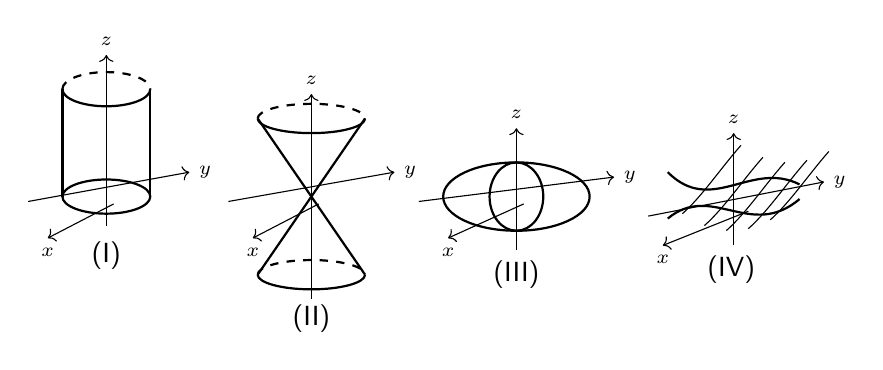
\begin{tikzpicture}[scale=0.62]
  % (I) cilindro
  \begin{scope}
    \draw[thick] (0,0) ellipse (0.9 and 0.35);
    \draw[thick] (-0.9,0) -- (-0.9,2.2);
    \draw[thick] (0.9,0) -- (0.9,2.2);
    \draw[thick] (-0.9,2.2) arc (180:360:0.9 and 0.35);
    \draw[thick,dashed] (-0.9,2.2) arc (180:0:0.9 and 0.35);
    \draw[->] (0,-0.6) -- (0,2.9) node[above]{\scriptsize$z$};
    \draw[->] (-1.6,-0.1) -- (1.7,0.5) node[right]{\scriptsize$y$};
    \draw[->] (0.15,-0.15) -- (-1.2,-0.85) node[below]{\scriptsize$x$};
    \node at (0,-1.2) {(I)};
  \end{scope}
  % (II) cono doble
  \begin{scope}[xshift=4.2cm]
    \draw[thick] (0,0) -- (-1.1,1.6); \draw[thick] (0,0) -- (1.1,1.6);
    \draw[thick] (-1.1,1.6) arc (180:360:1.1 and 0.3);
    \draw[thick,dashed] (-1.1,1.6) arc (180:0:1.1 and 0.3);
    \draw[thick] (0,0) -- (-1.1,-1.6); \draw[thick] (0,0) -- (1.1,-1.6);
    \draw[thick] (-1.1,-1.6) arc (180:360:1.1 and 0.3);
    \draw[thick,dashed] (-1.1,-1.6) arc (180:0:1.1 and 0.3);
    \draw[->] (0,-2.1) -- (0,2.1) node[above]{\scriptsize$z$};
    \draw[->] (-1.7,-0.1) -- (1.7,0.5) node[right]{\scriptsize$y$};
    \draw[->] (0.15,-0.15) -- (-1.2,-0.85) node[below]{\scriptsize$x$};
    \node at (0,-2.5) {(II)};
  \end{scope}
  % (III) elipsoide
  \begin{scope}[xshift=8.4cm]
    \draw[thick] (0,0) ellipse (1.5 and 0.7);
    \draw[thick] (0,0) ellipse (0.55 and 0.7);
    \draw[->] (0,-1.1) -- (0,1.4) node[above]{\scriptsize$z$};
    \draw[->] (-2.0,-0.1) -- (2.0,0.4) node[right]{\scriptsize$y$};
    \draw[->] (0.15,-0.15) -- (-1.4,-0.85) node[below]{\scriptsize$x$};
    \node at (0,-1.6) {(III)};
  \end{scope}
  % (IV) silla de montar
  \begin{scope}[xshift=12.8cm]
    \foreach \s in {-1.0,-0.55,-0.1,0.35,0.8}{
      \draw[thin] ({\s},{0.35*\s*\s-0.7}) .. controls ({\s+0.4},{0.35*\s*\s-0.35}) and ({\s+0.8},{0.35*\s*\s+0.25}) .. ({\s+1.2},{0.35*\s*\s+0.7});
    }
    \draw[thick] (-1.3,-0.45) .. controls (-0.4,0.3) and (0.4,-0.9) .. (1.4,-0.05);
    \draw[thick] (-1.3,0.5) .. controls (-0.4,-0.4) and (0.4,0.75) .. (1.4,0.25);
    \draw[->] (0.05,-1.0) -- (0.05,1.3) node[above]{\scriptsize$z$};
    \draw[->] (-1.7,-0.4) -- (1.9,0.3) node[right]{\scriptsize$y$};
    \draw[->] (0.35,-0.3) -- (-1.4,-1.0) node[below]{\scriptsize$x$};
    \node at (0,-1.5) {(IV)};
  \end{scope}
\end{tikzpicture}
\end{center}

\begin{center}
\begin{tabular}{|l|l|}
\hline
\textbf{Ecuaci\'on} & \textbf{Gr\'afica}\\
\hline
$x^2+4y^2+9z^2=1$ & (III) \\
\hline
$y=x^2-z^2$ & (IV) \\
\hline
$x^2+2z^2=1$ & (I) \\
\hline
$y^2=x^2+2z^2$ & (II) \\
\hline
\end{tabular}
\end{center}

\sol
\begin{itemize}[itemsep=1pt,topsep=2pt]
  \item $x^2+4y^2+9z^2=1$ es un \textbf{elipsoide} (los tres coeficientes son positivos y distintos): gr\'afica \textbf{(III)}.
  \item $y=x^2-z^2$ es un \textbf{paraboloide hiperb\'olico} (silla de montar), con eje en $y$: gr\'afica \textbf{(IV)}.
  \item $x^2+2z^2=1$ no involucra a $y$, por lo que es un \textbf{cilindro} el\'iptico con generatrices paralelas al eje $y$: gr\'afica \textbf{(I)}.
  \item $y^2=x^2+2z^2$ es un \textbf{cono} doble con eje en $y$: gr\'afica \textbf{(II)}.
\end{itemize}

\newpage
\examheader
\vspace{2pt}

\noindent\textbf{2.} (30\,\%) Una placa met\'alica ocupa la regi\'on del plano $D=\{(x,y)\in\mathbb{R}^2 : -5\leq x\leq 5,\ -5\leq y\leq 5\}$, donde $x$ y $y$ se miden en $cm$. La temperatura en todo punto $(x,y)\in D$, en grados Celsius, est\'a dada por la funci\'on $T(x,y)=20-4x^2-y^2$.

\begin{opciones}
  \item[a)] (15\,\%) ¿En qu\'e direcci\'on aumenta m\'as r\'apido la temperatura en el punto $A(2,3)$?, y ¿cu\'al es la tasa de crecimiento en dicho caso?
  \item[b)] (15\,\%) Encuentre la raz\'on de cambio de $T$ en el punto $P(1,2)$ en la direcci\'on que va de $P$ al punto $Q(2,1)$.
\end{opciones}

\sol \textbf{a)} $\nabla T(x,y) = (-8x,\,-2y)$, luego $\nabla T(2,3) = (-16,-6)$. La temperatura aumenta m\'as r\'apido en la direcci\'on del gradiente:
$$\hat u = \frac{(-16,-6)}{\sqrt{16^2+6^2}} = \frac{(-16,-6)}{\sqrt{292}} = \frac{(-16,-6)}{2\sqrt{73}},$$
y la tasa de crecimiento en esa direcci\'on es
$$\|\nabla T(2,3)\| = \sqrt{292} = 2\sqrt{73}\ {}^{\circ}\text{C/cm}.$$

\textbf{b)} $\nabla T(1,2) = (-8,-4)$. El vector de $P(1,2)$ a $Q(2,1)$ es $(1,-1)$, con norma $\sqrt2$; normalizado: $\hat v = \left(\frac{1}{\sqrt2},-\frac{1}{\sqrt2}\right)$. La raz\'on de cambio pedida es
$$D_{\hat v}T(1,2) = \nabla T(1,2)\cdot \hat v = (-8)\frac{1}{\sqrt2} + (-4)\left(-\frac{1}{\sqrt2}\right) = \frac{-8+4}{\sqrt2} = \frac{-4}{\sqrt2} = -2\sqrt2\ {}^{\circ}\text{C/cm}.$$

\bigskip
\noindent\textbf{3.} (30\,\%) Sea $g:\mathbb{R}^2\to\mathbb{R}$ una funci\'on diferenciable de las variables $u$ y $v$. Sea $f:\mathbb{R}^2\to\mathbb{R}$ la funci\'on definida por $f(x,y)=g(\operatorname{sen}x\cos y,\cos x\cos y)$. Encuentre la ecuaci\'on del plano tangente a la gr\'afica de $f$ en el punto $(\pi/2,\pi)$ si se sabe que:
\begin{romopc}
  \item $\overrightarrow{\nabla g}(\pi/2,\pi) = (-2,3)$ y $g(\pi/2,\pi)=-1$.
  \item $\overrightarrow{\nabla g}(-1,0) = (1,5)$ y $g(-1,0)=7$.
  \item $\overrightarrow{\nabla g}(1,0) = (-4,2)$ y $g(1,0)=0$.
\end{romopc}

\sol Sean $u=\operatorname{sen}x\cos y$ y $v=\cos x\cos y$. En el punto $(x,y)=(\pi/2,\pi)$:
$$u = \operatorname{sen}\left(\tfrac{\pi}{2}\right)\cos(\pi) = (1)(-1) = -1, \qquad v = \cos\left(\tfrac{\pi}{2}\right)\cos(\pi) = (0)(-1) = 0.$$
Como $(u,v)=(-1,0)$, el dato relevante es el (II): $\nabla g(-1,0)=(g_u,g_v)=(1,5)$ y $g(-1,0)=7$ (los datos I y III no se usan). Luego
$$f\left(\tfrac{\pi}{2},\pi\right) = g(-1,0) = 7.$$
Por la regla de la cadena, $f_x = g_u\,u_x + g_v\,v_x$ y $f_y = g_u\,u_y + g_v\,v_y$, con
$$u_x=\cos x\cos y,\quad v_x=-\operatorname{sen}x\cos y,\quad u_y=-\operatorname{sen}x\operatorname{sen}y,\quad v_y=-\cos x\operatorname{sen}y.$$
Evaluando en $(\pi/2,\pi)$: $\cos(\pi/2)=0$, $\operatorname{sen}(\pi/2)=1$, $\cos(\pi)=-1$, $\operatorname{sen}(\pi)=0$. As\'i,
$$u_x = 0, \qquad v_x = -(1)(-1) = 1, \qquad u_y = 0, \qquad v_y = 0.$$
Entonces
$$f_x\left(\tfrac{\pi}{2},\pi\right) = g_u\cdot 0 + g_v\cdot 1 = 5, \qquad f_y\left(\tfrac{\pi}{2},\pi\right) = g_u\cdot 0 + g_v\cdot 0 = 0.$$
La ecuaci\'on del plano tangente es
$$z = f\left(\tfrac{\pi}{2},\pi\right) + f_x\left(\tfrac{\pi}{2},\pi\right)\left(x-\tfrac{\pi}{2}\right) + f_y\left(\tfrac{\pi}{2},\pi\right)(y-\pi) = 7 + 5\left(x-\tfrac{\pi}{2}\right),$$
es decir,
$$z = 5x - \tfrac{5\pi}{2} + 7.$$

\vfill
\examfooter

\end{document}
